%!TEX root = ../dynamics.tex
\section{Analyzing the Features Affecting Batch Throughput}
\label{sec:throughput}
Next, we turn our attention to analyzing the factors that influence the progress (or the pace) of a batch, how those factors influence each other and how their importance changes over time. 

In order to conduct this analysis, we try to predict the throughput of a batch of tasks (or how many HITs get will get completed in the next time frame). 
The value we aim to predict is the batch \emph{throughput}, that is, the numbers of HITs that  will be completed for a given batch within the next time frame of 1 hour (i.e.,  the $DIFF\_HIT$ feature is a target class).
Specifically, we model this task as a regression problem using 29 features; some of them were used in the previous section to classify HIT type, we describe the remaining ones in Appendix A.

\subsection{Experimental Setup}

To predict the throughput of a batch at time $T$, we train a Random Forest Regression model with samples taken in the range $[T-\delta, T)$ where $\delta$ is the size of the time window that we are   considering directly prior to time $T$. The rational behind this approach is that the throughput should be directly correlated to the current and recent market situations. 
The research question we tackle in this context is:\\ \emph{``How much historical data does one need to consider to predict the throughput effectively?"}. \\ To answer this, we proceed by varying $\delta$.
To evaluate the effectiveness of $\delta$ values, we compute the coefficient of determination  $R^2$ \cite{sklearnweb, sklearn}.
In this experiment, we considered  data from June to October 2014 and hourly observations (see Section \ref{sec:tracker}), from which we uniformly sampled 50 time points for evaluation purposes. Finally, for each time point we considered a training time frame $\delta$ ranging from 1 hour to 24 hours. 

\subsection{Prediction}
In Figure \ref{fig:accuracy}, we observe that the computed evaluation score reaches its highest values when using the latest 4 hours as training time-frame, then decreases when we increase the training time-frame, to finally again increase and stabilize when we use up to 24 hours training data.
Note that the score is relatively low for batches with low throughput. 

Our prediction results (when using 4hours window) versus actual throughput values are shown in Figure \ref{fig:pred}. The prediction works best for larger batches having a large momentum as the Figure suggests.

\begin{figure}[tb]
	\centering
		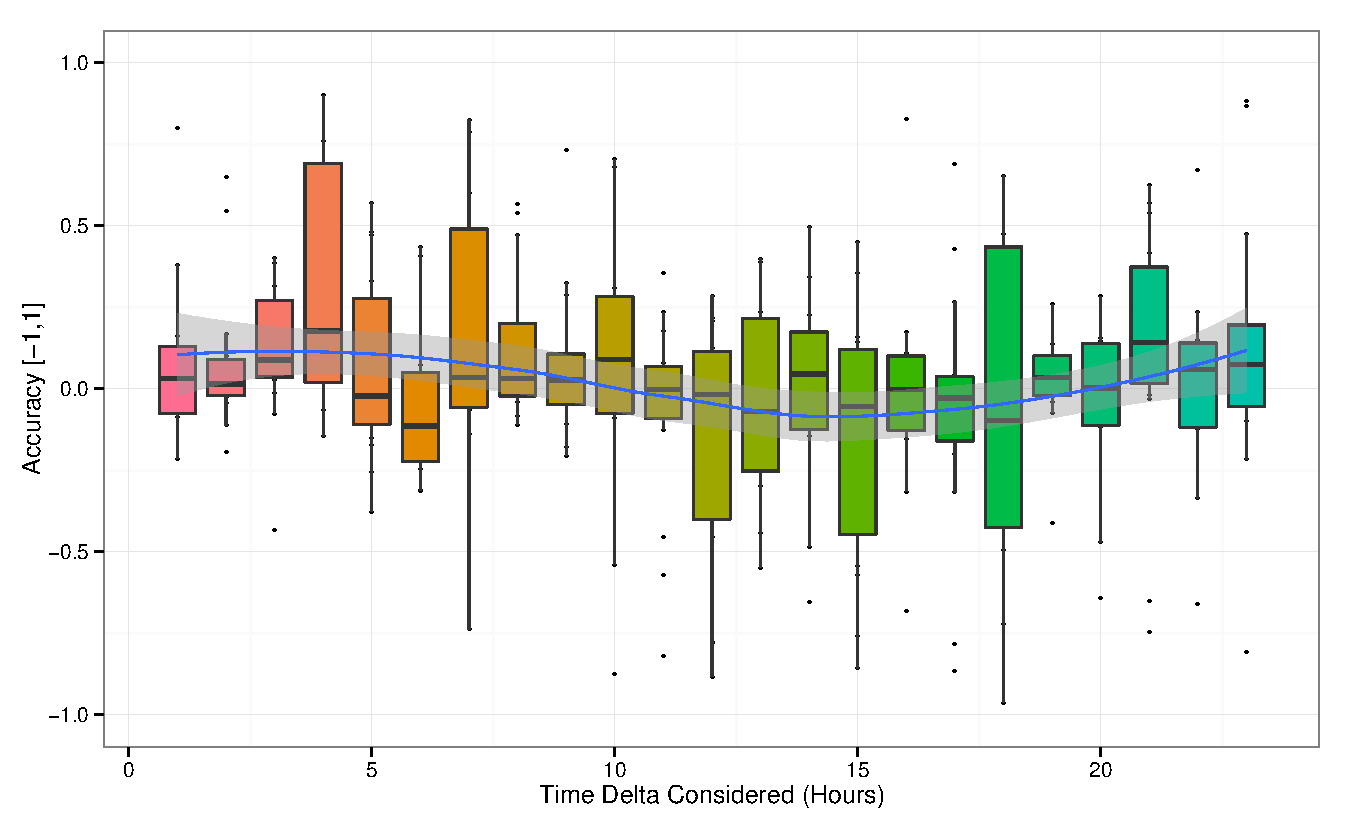
\includegraphics[width=0.48\textwidth]{figures/ML_accuracy}
	\caption{Score ($R^2$) of the throughput prediction when considering larger time spans as training sets. The red dots are average values, while the boxes represents the median, first and third quartiles. N.B., the implementation of the score function used in our experiments allows for negative values.}
	\label{fig:accuracy}
\end{figure}
\footnotetext{\url{http://scikit-learn.org/stable/modules/generated/sklearn.metrics.r2_score.html}}

\begin{figure}[tb]
	\centering
		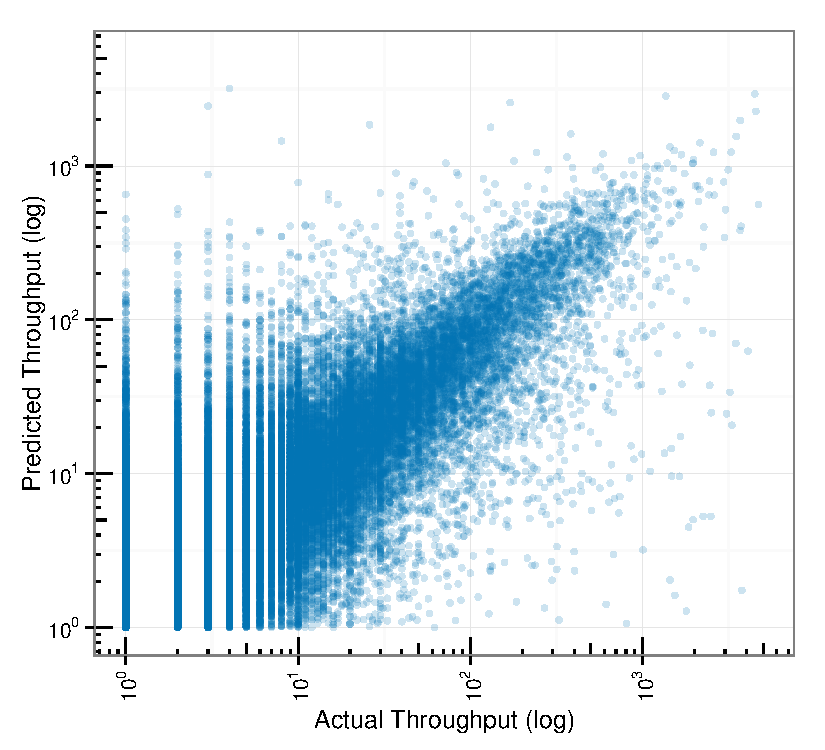
\includegraphics[width=0.48\textwidth]{figures/predictions_3}
	\caption{Prediction vs actual throughput values. Prediction is more accurate for larger throughput values. This suggests that the throughput will remain high until the batch gets smaller.}
	\label{fig:pred}
\end{figure}

\subsection{Features Importances}
In order to better grasp the characteristics of the batch throughput, we examine the prediction's features importances to understand which ones contributes more.

Figure \ref{fig:importances} shows the  contribution of the top 4 features and how it varies  when we increase the training time-frame. The rest of the features importances are listed in Table \ref{table:feats}, their slope indicates whether the feature is gaining importance overtime (positive value) or decreasing in importance (negative value).
The most important feature is $HIT\_Available$, that is, the current size of the batch. Indeed, as observed by previous work, larger batches tend to attract more workers \cite{mturk,crowddb}. This feature becomes less important when we consider longer periods, partly because of noise, but, most importantly, because of other features like $age\_minutes$ and $left\_minutes$, which encode additional facts and suggest that the crowd is sensitive to the newly posted HITs, or how \emph{fresh} the HITs are. To better understand this phenomenon, we conduct an analysis on what attracts the workforce to the the platform in the next section.

\begin{figure}[htb]
	\centering
		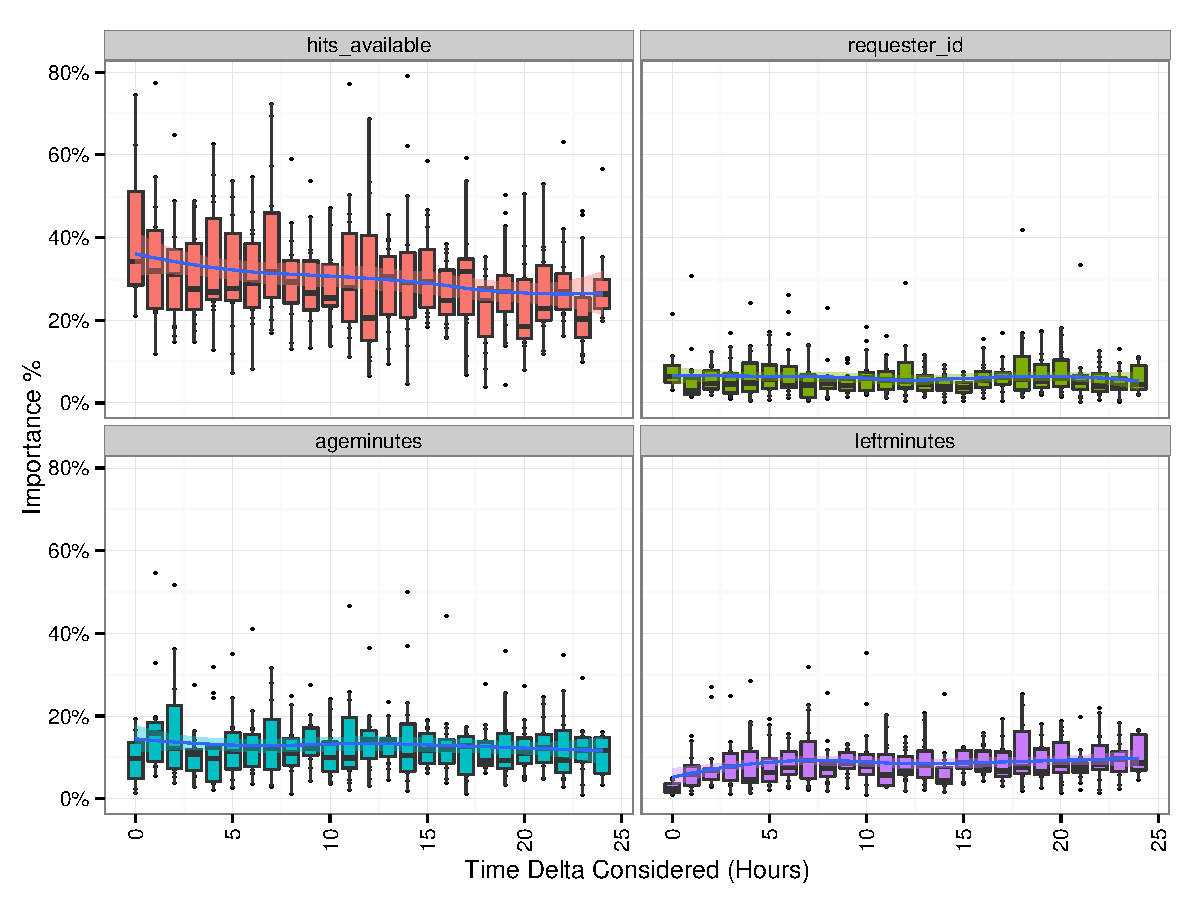
\includegraphics[width=0.5\textwidth]{figures/importances}
	\caption{Computed feature importance when considering larger training sets for the prediction.}
	\label{fig:importances}
\end{figure}


\begin{table}[ht]
\scriptsize
\begin{tabular}{|c|c|c|c|c|}
\hline
Feature              & mean      & stddev    & slope     & intercept \\
\hline
hits\_available      & 29.8606 & 13.4247 & -0.0257 & 34.4940 \\
ageminutes           & 12.9087 &  8.1967 & -0.0050 & 13.8181 \\
leftminutes          &  8.7300 &  5.5530 & 0.0061 & 7.6290 \\
requester\_id        &  6.2147 &  5.2943 & -0.0011 & 6.4305 \\
title                &  5.6441 &  4.2604 & -0.0033 & 6.2519 \\
description          &  4.8823 &  3.8975 & -0.0065 & 6.0617 \\
keywords             &  4.3765 &  3.3860 & -0.0074 & 5.7095 \\
time\_alloted        &  3.7994 &  3.6820 & -0.0010 & 3.9965 \\
reward               &  3.5439 &  2.7426 & -0.0011 & 3.7458 \\
totalapproved        &  2.5259 &  3.5108 & 0.0033 & 1.9311 \\
tasktype             &  2.1370 &  2.2673 & -0.0008 & 2.2986 \\
start\_time          &  1.2257 &  1.4123 & 0.0049 & 0.3325 \\
hitsAvailableUI      &  1.1428 &  1.2062 & 0.0039 & 0.4380 \\
diffHitsUI           &  1.0557 &  1.1237 & 0.0038 & 0.3568 \\
hitGroupsAvailableUI &  1.0438 &  1.0219 & 0.0034 & 0.4169 \\
diffGroupsUI         &  1.0408 &  1.0658 & 0.0030 & 0.4835 \\
master               &  0.9943 &  2.3816 & -0.0012 & 1.2134 \\
diffGroups           &  0.9660 &  0.9349 & 0.0032 & 0.3863 \\
rewardsArrived       &  0.9543 &  1.0710 & 0.0032 & 0.3698 \\
hitsCompleted        &  0.9293 &  0.9453 & 0.0031 & 0.3593 \\
percHitsCompleted    &  0.8974 &  0.8548 & 0.0030 & 0.3543 \\
location             &  0.8957 &  1.7592 & 0.0004 & 0.8184 \\
diffRewards          &  0.8920 &  0.8967 & 0.0023 & 0.4622 \\
rewardsCompleted     &  0.8890 &  0.8896 & 0.0026 & 0.4056 \\
percHitsPosted       &  0.8462 &  0.9552 & 0.0021 & 0.4618 \\
diffHits             &  0.8462 &  0.7514 & 0.0024 & 0.3972 \\
hitsArrived          &  0.7562 &  0.7946 & 0.0021 & 0.3760 \\
approvalrate         &  0.0000 &  0.0000 & 0 & 0 \\
\hline
\end{tabular}
\caption {Importances of the features used in the prediction experiment. A large mean indicates a better overall contribution to the prediction. A positive slope indicates that the feature is gaining in importance when the considered time window increases.}
\label{table:feats}
\end{table}